% ============================================================
%  08-chapitre2.tex  —  Spécification des besoins & Architecture
% ============================================================
\chapter{Spécification des besoins et architecture}

% ══════════════════════════════════════════════════════════════
\section{Capture des besoins}
% ══════════════════════════════════════════════════════════════

\subsection{Spécifications des besoins}

La spécification des besoins constitue la première étape du cycle de
développement d'une application. Elle doit définir clairement et
précisément l'application à concevoir. Pour la plateforme
\textbf{SolarEase}, ces besoins couvrent l'intégralité du cycle métier
d'une société d'installation photovoltaïque, depuis l'acquisition d'un
nouveau prospect jusqu'à l'archivage du projet réalisé. Ils se
répartissent en deux catégories~: \textbf{fonctionnels} et
\textbf{non fonctionnels}.

\subsection{Identification des acteurs}

Dans ce qui suit, nous décrivons les différents acteurs qui interagissent
avec notre système. Cette identification permet non seulement de définir
les limites du système, mais aussi de mieux comprendre les rôles et les
besoins spécifiques de chaque utilisateur. Ainsi, la plateforme SolarEase
sera utilisée par quatre types d'acteurs.

\begin{itemize}[leftmargin=2em, label={$\blacktriangleright$}]
  \item \textbf{Administrateur~:} il assure la gestion et la
    configuration globale de la plateforme. Il est responsable de la
    création et de la gestion des comptes installateurs, du catalogue
    d'équipements (panneaux solaires, onduleurs, Night~Panels), du
    traitement des demandes publiques, de l'affectation des projets aux
    installateurs et du suivi global de l'activité.

  \item \textbf{Installateur~:} il s'agit de l'acteur métier principal
    de la plateforme. Représentant une société d'installation
    photovoltaïque, il gère ses clients, crée et suit ses projets
    solaires, lance les calculs de dimensionnement, génère les rapports
    techniques au format PDF, met à jour l'avancement terrain, échange
    en temps réel avec ses clients via la messagerie projet, et produit
    les devis et factures associés.

  \item \textbf{Client final~:} bénéficiaire de la solution
    photovoltaïque, il dispose d'un espace dédié. Il s'inscrit en
    validant un code OTP envoyé par e-mail, consulte l'avancement de
    ses projets, télécharge les rapports techniques et les documents
    (PDF, factures), accepte ou refuse les devis, soumet de nouvelles
    demandes et échange avec son installateur via la messagerie
    intégrée.

  \item \textbf{Visiteur~:} il s'agit d'un utilisateur non authentifié
    qui peut consulter les informations publiques de la plateforme
    SolarEase et soumettre une demande de contact (étude, devis,
    renseignement) via le formulaire public. Une fois la demande
    validée, le visiteur peut être promu au rang de client par
    l'administrateur.
\end{itemize}

\subsection{Besoins fonctionnels}

Les besoins fonctionnels décrivent les actions spécifiques que le système
doit permettre aux utilisateurs d'accomplir. Conformément à
l'identification des acteurs (section~2.1.2), la liste ci-dessous regroupe
les fonctionnalités attendues \textbf{par acteur}, afin de relier chaque
besoin au profil qui l'exerce. Les fonctions d'authentification communes
(JWT, profil, mot de passe) sont rappelées pour les acteurs authentifiés
concernés.

\begin{itemize}[leftmargin=1.6em, label={$\bullet$}]

  \item \textbf{Visiteur (utilisateur non authentifié)}
  \begin{itemize}[leftmargin=2em, label={--}]
    \item Consulter les informations publiques de la plateforme (présentation,
      simulateur, tarifs, contact).
    \item Soumettre une demande solaire via le formulaire de contact public
      (étude, devis, renseignement).
  \end{itemize}

  \item \textbf{Client final (\texttt{CLIENT})}
  \begin{itemize}[leftmargin=2em, label={--}]
    \item S'inscrire avec vérification par code OTP envoyé par e-mail.
    \item S'authentifier par JWT (\textit{access~token}~+~\textit{refresh~token}).
    \item Renvoyer un code OTP en cas d'expiration.
    \item Consulter et mettre à jour son profil utilisateur.
    \item Changer son mot de passe.
    \item Consulter son tableau de bord (projets, devis, factures, demandes).
    \item Visualiser le détail d'un projet (avancement, documents).
    \item Télécharger les rapports PDF de dimensionnement et les factures.
    \item Accepter ou refuser un devis reçu de l'installateur (génération
      automatique d'une facture en cas d'acceptation).
    \item Recevoir automatiquement la facture PDF par e-mail (workflow n8n
      déclenché à l'acceptation du devis ou à la clôture du projet).
    \item Soumettre une nouvelle demande depuis l'espace client authentifié.
    \item Échanger avec l'installateur via la messagerie projet.
    \item Recevoir des notifications temps réel (WebSocket / STOMP) et les
      consulter dans un centre de notifications (marquage lu / non lu).
  \end{itemize}

  \item \textbf{Installateur (\texttt{INSTALLER})}
  \begin{itemize}[leftmargin=2em, label={--}]
    \item S'authentifier par JWT et gérer son profil (consultation, mise à jour,
      changement de mot de passe).
    \item Consulter la liste de ses clients (pagination, recherche par nom
      ou e-mail).
    \item Ajouter, modifier et supprimer un client.
    \item Consulter la liste de ses projets et le tableau de bord associé.
    \item Créer un projet (client, localisation, type, puissance, budget).
    \item Modifier les informations d'un projet qui lui est affecté.
    \item Suivre l'évolution d'un projet à travers six statuts
      (\texttt{CREATED}, \texttt{EN\_PREPARATION},
      \texttt{INSTALLATEUR\_AFFECTE}, \texttt{IN\_PROGRESS},
      \texttt{COMPLETED}, \texttt{CANCELLED}).
    \item Mettre à jour le pourcentage d'avancement terrain (commentaire
      inclus).
    \item Lancer un dimensionnement standard (données PVGIS, Commission
      Européenne).
    \item Lancer un dimensionnement Night~Panel (production nocturne complémentaire,
      concept R\&D)~;
    \item Comparer les scénarios Classique vs Night~Panel (courbes sur
      24~heures).
    \item Consulter l'analyse financière (ROI, \textit{payback}, flux cumulés
      sur 25~ans).
    \item Obtenir une recommandation IA contextualisée (Ollama / TinyLLaMA,
      enrichie par RAG hybride~: catalogue société + recherche sémantique
      \texttt{pgvector} sur normes STEG/ANME).
    \item Générer et télécharger un rapport PDF (synthèse technique, schémas,
      courbes, recommandation IA).
    \item Consulter le catalogue d'équipements (panneaux, onduleurs,
      Night~Panels).
    \item Créer un devis associé à un projet et l'envoyer au client par
      notification.
    \item Consulter la liste de ses devis et factures.
    \item Échanger avec le client via la messagerie projet et recevoir des
      notifications temps réel.
  \end{itemize}

  \item \textbf{Administrateur (\texttt{ADMIN})}
  \begin{itemize}[leftmargin=2em, label={--}]
    \item S'authentifier par JWT et gérer son profil (consultation, mise à jour,
      changement de mot de passe).
    \item Créer les comptes installateurs (compte vérifié d'office, rôle
      \texttt{INSTALLER}).
    \item Gérer les rôles utilisateurs (\texttt{CLIENT}, \texttt{INSTALLER},
      \texttt{ADMIN}).
    \item Consulter le tableau de bord global avec indicateurs KPI (vue
      transverse sur projets, clients, demandes).
    \item Consulter, filtrer et trier l'ensemble des demandes solaires.
    \item Assigner une demande à un administrateur.
    \item Promouvoir un prospect (visiteur) au rang de client.
    \item Convertir une demande en projet.
    \item Affecter un installateur à un projet.
    \item Superviser l'ensemble des clients, projets, devis et factures
      (CRUD et recherche, sans restriction d'affectation).
    \item Administrer le catalogue d'équipements~: ajouter, modifier,
      supprimer, activer ou désactiver un équipement.
    \item Accéder à l'ensemble des fonctionnalités installateur (dimensionnement,
      PDF, suivi terrain, messagerie) sur l'ensemble des projets.
  \end{itemize}

  \item \textbf{Besoins transverses (plateforme et déploiement)}
  \begin{itemize}[leftmargin=2em, label={--}]
    \item Contrôle d'accès centralisé au niveau de l'API~Gateway selon le
      rôle porté par le JWT.
    \item Conteneurisation des microservices avec \textbf{Docker}
      (Dockerfile multi-stage).
    \item Orchestration locale via \textbf{Docker~Compose}.
    \item Déploiement continu via \textbf{GitHub~Actions} et
      \textbf{Microsoft Azure} (VM + Docker Compose)~; frontend sur
      \textbf{Vercel}.
    \item Automatisation des notifications métier via \textbf{n8n}
      (webhook interne, envoi SMTP des factures PDF au client).
  \end{itemize}

\end{itemize}

\subsection{Besoins non fonctionnels}

Les besoins non fonctionnels se réfèrent à la qualité globale du système.
Voici les principaux critères retenus pour la plateforme SolarEase~:

\begin{itemize}[leftmargin=1.6em, label={--}]
  \item \textbf{Sécurité des données utilisateurs~:} la sécurité de la
    plateforme est assurée par un mécanisme d'authentification en deux
    étapes combinant \textbf{JWT} (\textit{access~token} et
    \textit{refresh~token}) et vérification par code OTP à l'inscription.
    Le contrôle d'accès est centralisé au niveau d'un \textbf{API~Gateway}
    qui valide chaque requête en fonction du rôle de l'utilisateur,
    garantissant ainsi la confidentialité et l'intégrité des informations.

  \item \textbf{Maintenabilité~:} le code est structuré en
    \textbf{microservices} indépendants (\textit{Identity}, \textit{Project},
    \textit{Dimensioning}, \textit{Gateway}), respectant le principe de
    séparation des responsabilités. L'utilisation d'un outil de versioning
    \textbf{Git/GitHub} permet de garder la trace de toutes les évolutions,
    et une couverture de tests automatisés ($\geq 80\,\%$) facilite la
    détection des régressions.

  \item \textbf{Ergonomie~:} la plateforme propose une interface
    utilisateur conviviale et intuitive, construite avec \textbf{React~18},
    \textbf{TailwindCSS} et \textbf{Radix~UI}. Elle permet une prise en
    main aisée sans formation préalable, grâce à des composants
    réutilisables et des écrans cohérents.

  \item \textbf{Performance~:} le temps de réponse moyen des API est
    maintenu en dessous de \textbf{500\,ms} pour les opérations CRUD, et
    en dessous de \textbf{3~secondes} pour un dimensionnement complet
    (incluant l'appel PVGIS et la génération IA). Le cache du frontend
    (\textit{TanStack~Query}) limite les appels réseau redondants.

  \item \textbf{Scalabilité~:} l'architecture microservices permet la
    montée en charge indépendante de chaque service. \textbf{PostgreSQL}
    est déployé en mode \textit{database-per-service} pour éviter les
    goulots d'étranglement, et le frontend est livré en continu sur
    \textbf{Vercel}.

  \item \textbf{Disponibilité~:} la résilience est assurée par des
    mécanismes de \textbf{fallback}~: en cas d'indisponibilité de l'API
    PVGIS, le système bascule sur un calcul de repli~; en cas
    d'indisponibilité du service Ollama, la recommandation IA est
    désactivée sans bloquer le dimensionnement.

  \item \textbf{Portabilité~:} l'ensemble de la solution est conteneurisé
    via \textbf{Docker} et orchestré par \textbf{Docker~Compose}. Toutes
    les configurations sensibles sont externalisées dans des variables
    d'environnement, permettant un déploiement reproductible sur
    n'importe quel environnement (local, staging, production).

  \item \textbf{Flexibilité~:} l'utilisateur peut revenir au tableau de
    bord depuis n'importe quelle interface ou section de l'application,
    assurant ainsi une navigation fluide et intuitive grâce à un menu
    latéral persistant.
\end{itemize}

% ══════════════════════════════════════════════════════════════
\section{Modélisation des besoins~: diagramme de cas d'utilisation général}
% ══════════════════════════════════════════════════════════════

Dans le cadre du développement de la plateforme SolarEase, un diagramme
de cas d'utilisation global a été conçu afin de représenter les
principales interactions entre le système et les quatre profils
d'utilisateurs (Administrateur, Installateur, Client final et Visiteur).
Il permet de visualiser clairement les fonctionnalités offertes à chaque
acteur ainsi que les relations d'inclusion et d'extension entre les
différents cas d'utilisation (figure~\ref{fig:uml-global}).

\begin{figure}[H]
  \centering
  \IfFileExists{UseCaseDiagram1.png}{%
    \includegraphics[width=0.85\textwidth]{UseCaseDiagram1.png}%
  }{%
    \fbox{\parbox{0.85\textwidth}{\centering Diagramme manquant\\(UseCaseDiagram1.png)}}%
  }
  \caption{Diagramme de cas d'utilisation général de SolarEase}
  \label{fig:uml-global}
\end{figure}

% ══════════════════════════════════════════════════════════════
\section{Pilotage du projet avec Kanban}
% ══════════════════════════════════════════════════════════════

Dans le cadre du projet SolarEase, le pilotage a été réalisé avec la méthode
\textbf{Kanban}. Ce choix permet de visualiser l'avancement en continu, de
prioriser les tâches selon leur valeur métier et de limiter le travail en
cours (\textit{WIP limit}) afin de maintenir un flux de livraison stable.

\subsection{Équipe et rôles}

L'équipe projet est organisée autour des rôles suivants~:

\begin{table}[H]
  \centering
  \caption{Rôles et responsabilités de l'équipe projet}
  \label{tab:equipe}
  \small
  \renewcommand{\arraystretch}{1.3}
  \begin{tabularx}{\textwidth}{@{}>{\bfseries}L{4.5cm} X@{}}
    \toprule
    \multicolumn{2}{@{}l}{\theadrow \thead{Équipe projet SolarEase}} \\
    \midrule
    Product Owner &
      Définit la vision produit, gère et priorise le Product Backlog,
      valide les incréments livrés et arbitre les choix fonctionnels en
      lien avec les parties prenantes métier. Rôle assuré par l'auteur
      dans le cadre du PFE. \\
    \addlinespace
    Développeur full-stack &
      Conçoit et implémente les fonctionnalités Frontend
      (React~/~TypeScript) et Backend (Spring~Boot, microservices), met
      en place la base de données, écrit les tests, prépare les
      livrables et déploie les incréments. Rôle assuré par l'auteur. \\
    \addlinespace
    Scrum Master / Référent Kanban &
      Anime le flux Kanban, veille au respect des limites WIP, organise
      les revues d'incrément et alimente le tableau Jira. Rôle assuré
      par l'auteur. \\
    \addlinespace
    Encadrant pédagogique &
      M.~Aymen Waheb. Assure le suivi académique du PFE, valide les
      orientations méthodologiques et techniques, anime les revues de
      fin de sprint. Considéré comme partie prenante externe et non
      comme membre opérationnel de l'équipe. \\
    \bottomrule
  \end{tabularx}
\end{table}

\subsection{Organisation du flux Kanban}

Le suivi opérationnel est assuré sur un tableau Kanban (\textit{Jira}) avec les
colonnes suivantes~:

\begin{enumerate}
  \item \textbf{To Do} -- tâches priorisées, prêtes à être démarrées~;
  \item \textbf{In Progress} -- tâches en cours de développement (WIP $\leq$ 3)~;
  \item \textbf{Review} -- tâches en relecture de code ou validation fonctionnelle~;
  \item \textbf{Done} -- tâches terminées, testées et validées.
\end{enumerate}

Cette organisation a facilité~:
\begin{itemize}
  \item la visibilité quotidienne sur le travail en cours~;
  \item la détection rapide des blocages~;
  \item l'ajustement des priorités en continu grâce au flux tiré.
\end{itemize}

\subsection{Product Backlog}

Le Product Backlog regroupe l'ensemble des User Stories identifiées, classées
par priorité et rattachées à un sprint de livraison.

\begin{table}[H]
  \caption{Product Backlog SolarEase}
  \label{tab:backlog}
  \centering
  \small
  \begin{tabularx}{\textwidth}{|C{1cm}|L{2cm}|X|C{1.4cm}|C{1.4cm}|C{1cm}|}
    \hline
    \rowcolor{figblue}
    \textcolor{white}{\textbf{ID}} &
    \textcolor{white}{\textbf{Acteur}} &
    \textcolor{white}{\textbf{User Story}} &
    \textcolor{white}{\textbf{Sprint}} &
    \textcolor{white}{\textbf{Priorité}} &
    \textcolor{white}{\textbf{Effort}} \\
    \hline
    \rowcolor{gray!5}
    US-01 & Client & M'inscrire et recevoir un OTP de confirmation par e-mail & Sprint 1 & \textcolor{red}{\textbf{Haute}} & 5 \\
    \hline
    US-02 & Utilisateur & Me connecter et obtenir un JWT sécurisé & Sprint 1 & \textcolor{red}{\textbf{Haute}} & 5 \\
    \hline
    \rowcolor{gray!5}
    US-03 & Utilisateur & Gérer mon profil utilisateur (infos, mot de passe) & Sprint 1 & Moyenne & 3 \\
    \hline
    US-04 & Installateur & Créer, modifier et supprimer mes clients & Sprint 2 & \textcolor{red}{\textbf{Haute}} & 5 \\
    \hline
    \rowcolor{gray!5}
    US-05 & Installateur & Visualiser un tableau de bord avec KPI & Sprint 2 & Moyenne & 5 \\
    \hline
    US-06 & Installateur & Créer et suivre mes projets solaires & Sprint 3 & \textcolor{red}{\textbf{Haute}} & 8 \\
    \hline
    \rowcolor{gray!5}
    US-07 & Admin & Gérer le catalogue d'équipements (panneaux, onduleurs) & Sprint 3 & Moyenne & 5 \\
    \hline
    US-08 & Installateur & Lancer un dimensionnement automatique (PVGIS) & Sprint 4 & \textcolor{red}{\textbf{Haute}} & 13 \\
    \hline
    \rowcolor{gray!5}
    US-09 & Installateur & Simuler un scénario Night Panel (production nocturne) & Sprint 4 & \textcolor{red}{\textbf{Haute}} & 8 \\
    \hline
    US-10 & Installateur & Comparer les scénarios (Classique vs Night Panel) & Sprint 4 & \textcolor{red}{\textbf{Haute}} & 5 \\
    \hline
    \rowcolor{gray!5}
    US-11 & Installateur & Générer un rapport PDF professionnel & Sprint 5 & \textcolor{red}{\textbf{Haute}} & 5 \\
    \hline
    US-12 & Installateur & Recevoir une recommandation IA contextualisée & Sprint 5 & Moyenne & 5 \\
    \hline
    \rowcolor{gray!5}
    US-13 & Installateur & Consulter l'analyse financière (ROI, payback, cash-flow) & Sprint 5 & \textcolor{red}{\textbf{Haute}} & 5 \\
    \hline
    US-14 & Client final & Consulter mes projets et documents en ligne & Sprint 5 & Moyenne & 5 \\
    \hline
  \end{tabularx}
\end{table}

\subsection{Planification des sprints}

Le projet est découpé en \textbf{cinq sprints} organisés selon le flux
Kanban. Chaque sprint correspond à un ensemble cohérent de fonctionnalités
tirées du Backlog et livrées de manière incrémentale~:

\begin{table}[H]
  \caption{Planification des sprints Kanban}
  \label{tab:sprints}
  \centering
  \begin{tabularx}{\textwidth}{|C{1.6cm}|L{4.2cm}|X|C{1.8cm}|}
    \hline
    \rowcolor{figblue}
    \textcolor{white}{\textbf{Sprint}} &
    \textcolor{white}{\textbf{Objectif}} &
    \textcolor{white}{\textbf{User Stories}} &
    \textcolor{white}{\textbf{Durée}} \\
    \hline
    Sprint 1 & Authentification et profil utilisateur & US-01, US-02, US-03 & 2 semaines \\
    \hline
    \rowcolor{gray!5}
    Sprint 2 & Gestion des clients et tableau de bord & US-04, US-05 & 2 semaines \\
    \hline
    Sprint 3 & Gestion des projets et catalogue & US-06, US-07 & 2 semaines \\
    \hline
    \rowcolor{gray!5}
    Sprint 4 & Dimensionnement PVGIS, Night Panel et comparaison & US-08, US-09, US-10 & 2 semaines \\
    \hline
    Sprint 5 & PDF, recommandation IA, finance et espace client & US-11, US-12, US-13, US-14 & 2 semaines \\
    \hline
  \end{tabularx}
\end{table}

\noindent La figure~\ref{fig:timeline} illustre la répartition temporelle
des cinq sprints, regroupés en deux chapitres de réalisation.

\begin{figure}[H]
  \centering
  \begin{tikzpicture}[
    iter/.style={draw=isetblue, fill=lightblue, rounded corners=3pt,
                   minimum height=0.9cm, font=\footnotesize\bfseries,
                   align=center},
    rel/.style={draw=isetblue!60, dashed, thick, rounded corners=5pt}]
    \draw[->, thick, gray] (0,0) -- (14.5,0) node[right]{\footnotesize Temps};
    \node[iter, minimum width=2.4cm] at (1.2,0.6) {Sprint 1};
    \node[iter, minimum width=2.4cm] at (3.8,0.6) {Sprint 2};
    \node[iter, minimum width=2.4cm] at (6.4,0.6) {Sprint 3};
    \node[iter, minimum width=2.4cm] at (9.0,0.6) {Sprint 4};
    \node[iter, minimum width=2.4cm] at (11.6,0.6) {Sprint 5};
    \node[font=\tiny, below] at (1.2,-0.1) {Sem. 1--2};
    \node[font=\tiny, below] at (3.8,-0.1) {Sem. 3--4};
    \node[font=\tiny, below] at (6.4,-0.1) {Sem. 5--6};
    \node[font=\tiny, below] at (9.0,-0.1) {Sem. 7--8};
    \node[font=\tiny, below] at (11.6,-0.1) {Sem. 9--10};
    \node[font=\tiny, above, isetblue] at (1.2,1.15) {Auth};
    \node[font=\tiny, above, isetblue] at (3.8,1.15) {Clients};
    \node[font=\tiny, above, isetblue] at (6.4,1.15) {Dimensionn.};
    \node[font=\tiny, above, isetblue] at (9.0,1.15) {Collab.};
    \node[font=\tiny, above, isetblue] at (11.6,1.15) {Commercial};
    % Chapitre groupings (Chap 3 = Sprints 1-2, Chap 4 = Sprints 3-5)
    \draw[rel] (-0.3,-0.5) rectangle (5.2,1.6);
    \node[font=\footnotesize\bfseries, isetblue] at (2.4,-0.8) {Chapitre 3 -- Sprints 1 et 2};
    \draw[rel] (4.9,-0.5) rectangle (13.1,1.6);
    \node[font=\footnotesize\bfseries, isetblue] at (9.0,-0.8) {Chapitre 4 -- Sprints 3, 4 et 5};
  \end{tikzpicture}
  \caption{Timeline du projet SolarEase (5 sprints Kanban répartis en 2 chapitres)}
  \label{fig:timeline}
\end{figure}

Chaque sprint suit le cycle Kanban suivant~:
\begin{enumerate}
  \item \textbf{Sélection~:} les User Stories les plus prioritaires sont tirées du Backlog~;
  \item \textbf{Développement~:} flux continu avec limite WIP (Work In Progress)~;
  \item \textbf{Revue~:} démonstration de l'incrément et validation
    fonctionnelle avec l'encadrant pédagogique (M.~Aymen Waheb), à la
    fin de chaque sprint~;
  \item \textbf{Rétrospective~:} identification des améliorations pour le sprint suivant.
\end{enumerate}

% ══════════════════════════════════════════════════════════════
\section{Architecture technique globale}
% ══════════════════════════════════════════════════════════════

\subsection{Choix de l'architecture microservices}

L'architecture \textbf{microservices} a été adoptée pour les raisons suivantes~:
\begin{itemize}
  \item \textbf{Découplage}~: chaque service est indépendant et dispose de sa
    propre base de données (\textit{database-per-service pattern})~;
  \item \textbf{Scalabilité}~: un service peut être mis à l'échelle
    indépendamment sans impacter les autres~;
  \item \textbf{Maintenabilité}~: les équipes peuvent travailler sur des services
    distincts sans conflits~;
  \item \textbf{Résilience}~: la défaillance d'un service n'entraîne pas
    l'arrêt complet de la plateforme.
\end{itemize}

\subsection{Schéma d'architecture globale}

La figure~\ref{fig:architecture} présente la vue d'ensemble de l'architecture.
Le Frontend communique exclusivement avec l'API Gateway, qui route les requêtes
vers le service approprié. Chaque microservice dispose de sa propre base de
données PostgreSQL (\textit{database-per-service}) et le Dimensioning Service
accède à deux services externes~: l'API PVGIS pour les données d'irradiation
et le modèle Ollama pour les recommandations IA.

\begin{figure}[H]
  \centering
  \resizebox{0.95\textwidth}{!}{%
  \begin{tikzpicture}[
      node distance=0.8cm,
      svc/.style={draw=isetblue, fill=lightblue, rounded corners,
                  minimum width=3cm, minimum height=0.9cm,
                  font=\footnotesize\bfseries, align=center},
      db/.style={draw=isetgold!80!black, fill=isetgold!20, rounded corners=2pt,
                 minimum width=3cm, minimum height=0.6cm,
                 font=\scriptsize, align=center},
      ext/.style={draw=green!60!black, fill=green!10, rounded corners,
                  minimum width=2.2cm, minimum height=0.6cm,
                  font=\scriptsize\bfseries, align=center}]

    % ── Frontend ──
    \node[svc, fill=isetgold!30, minimum width=8cm] (fe)
      {Frontend React 18 (Port 3000)};

    % ── Gateway ──
    \node[svc, fill=isetblue, text=white, below=0.8cm of fe, minimum width=8cm] (gw)
      {API Gateway (Port 8080)};

    % ── Services (espacement réduit) ──
    \node[svc, below left=1.2cm and 1.8cm of gw] (id)
      {Identity Service\\(8081)};
    \node[svc, below=1.2cm of gw] (ps)
      {Project Service\\(8082)};
    \node[svc, below right=1.2cm and 1.8cm of gw] (ds)
      {Dimensioning\\Service (8083)};

    % ── Bases de données ──
    \node[db, below=0.6cm of id] (dbi) {PostgreSQL\\solarease\_identity};
    \node[db, below=0.6cm of ps] (dbp) {PostgreSQL\\solarease\_projects};
    \node[db, below=0.6cm of ds] (dbd) {PostgreSQL\\solarease\_dim};

    % ── Services externes (sous la BDD dim) ──
    \node[ext, below left=0.6cm and -0.4cm of dbd] (pvgis) {PVGIS API};
    \node[ext, below right=0.6cm and -0.4cm of dbd] (ollama) {Ollama LLM};

    % ── Flèches ──
    \draw[->, thick] (fe) -- (gw);
    \draw[->, isetblue] (gw) -- (id);
    \draw[->, isetblue] (gw) -- (ps);
    \draw[->, isetblue] (gw) -- (ds);
    \draw[->, gray] (id) -- (dbi);
    \draw[->, gray] (ps) -- (dbp);
    \draw[->, gray] (ds) -- (dbd);
    \draw[->, green!60!black, dashed] (dbd) -- (pvgis);
    \draw[->, green!60!black, dashed] (dbd) -- (ollama);

  \end{tikzpicture}%
  }
  \caption{Architecture microservices de SolarEase}
  \label{fig:architecture}
\end{figure}

\subsection{Flux de sécurité}

Le flux de sécurité centralisé fonctionne ainsi~:
\begin{enumerate}
  \item Le client envoie une requête avec l'en-tête \texttt{Authorization: Bearer <JWT>}~;
  \item Le Gateway valide le token JWT (signature + expiration)~;
  \item Si valide, il extrait les informations utilisateur et les propage
    via des en-têtes internes (\texttt{X-User-Id}, \texttt{X-User-Role})~;
  \item Les services métiers exploitent ces en-têtes internes sur le réseau de confiance, sans revalider le JWT~;
  \item Si le token est expiré, le client utilise le refresh token pour en obtenir un nouveau.
\end{enumerate}

\subsection{Stack technique}

Le choix technologique de SolarEase repose sur des outils modernes, éprouvés
et adaptés au contexte microservices. Le tableau~\ref{tab:stack} détaille
chaque couche.

\begin{table}[H]
  \caption{Stack technique de SolarEase}
  \label{tab:stack}
  \centering
  \small
  \begin{tabularx}{\textwidth}{|L{2.8cm}|L{4.2cm}|X|}
    \hline
    \rowcolor{figblue}
    \textcolor{white}{\textbf{Couche}} &
    \textcolor{white}{\textbf{Technologie}} &
    \textcolor{white}{\textbf{Justification}} \\
    \hline
    \multicolumn{3}{|l|}{\cellcolor{gray!8}\textbf{\footnotesize Backend}} \\
    \hline
    Langage \& Framework & Spring Boot 3.2 / Java 17 & Écosystème mature, support natif microservices, Spring Security intégré \\
    \hline
    Gateway & Spring Cloud Gateway & Routage centralisé, filtres JWT, load-balancing \\
    \hline
    Base de données & PostgreSQL 16 & Robustesse ACID, support JSON natif, extensibilité \\
    \hline
    Sécurité & JWT + OTP + Spring Security & Architecture stateless, vérification en deux étapes \\
    \hline
    Intelligence artificielle & Ollama / TinyLLaMA & LLM local, autonomie totale, pas de dépendance cloud \\
    \hline
    API externe & PVGIS v5.2 (UE) & Données d'irradiation officielles, gratuites et fiables \\
    \hline
    \multicolumn{3}{|l|}{\cellcolor{gray!8}\textbf{\footnotesize Frontend}} \\
    \hline
    Framework UI & React 18 / TypeScript & Typage fort, composants réutilisables, écosystème riche \\
    \hline
    Build & Vite 5 & Compilation ultra-rapide, HMR instantané \\
    \hline
    Styling & TailwindCSS v4 + Radix UI & Design system cohérent, composants accessibles \\
    \hline
    Gestion d'état & Zustand + TanStack Query & État global léger, cache serveur intelligent \\
    \hline
    Formulaires & React Hook Form + Zod & Validation typée côté client, performances optimales \\
    \hline
    \multicolumn{3}{|l|}{\cellcolor{gray!8}\textbf{\footnotesize DevOps \& Outils}} \\
    \hline
    Conteneurisation & Docker + Docker Compose & Portabilité, déploiement reproductible \\
    \hline
    Gestion de projet & Jira (Kanban) & Suivi visuel, priorisation continue \\
    \hline
    Versioning & Git + GitHub & Collaboration, traçabilité du code \\
    \hline
  \end{tabularx}
\end{table}

\subsection{Modèle de données globale}

Le diagramme de classes ci-dessous présente la modélisation statique du système
SolarEase. Il regroupe les entités principales de chaque microservice ainsi que
leurs relations (associations, compositions).

\begin{figure}[H]
  \centering
  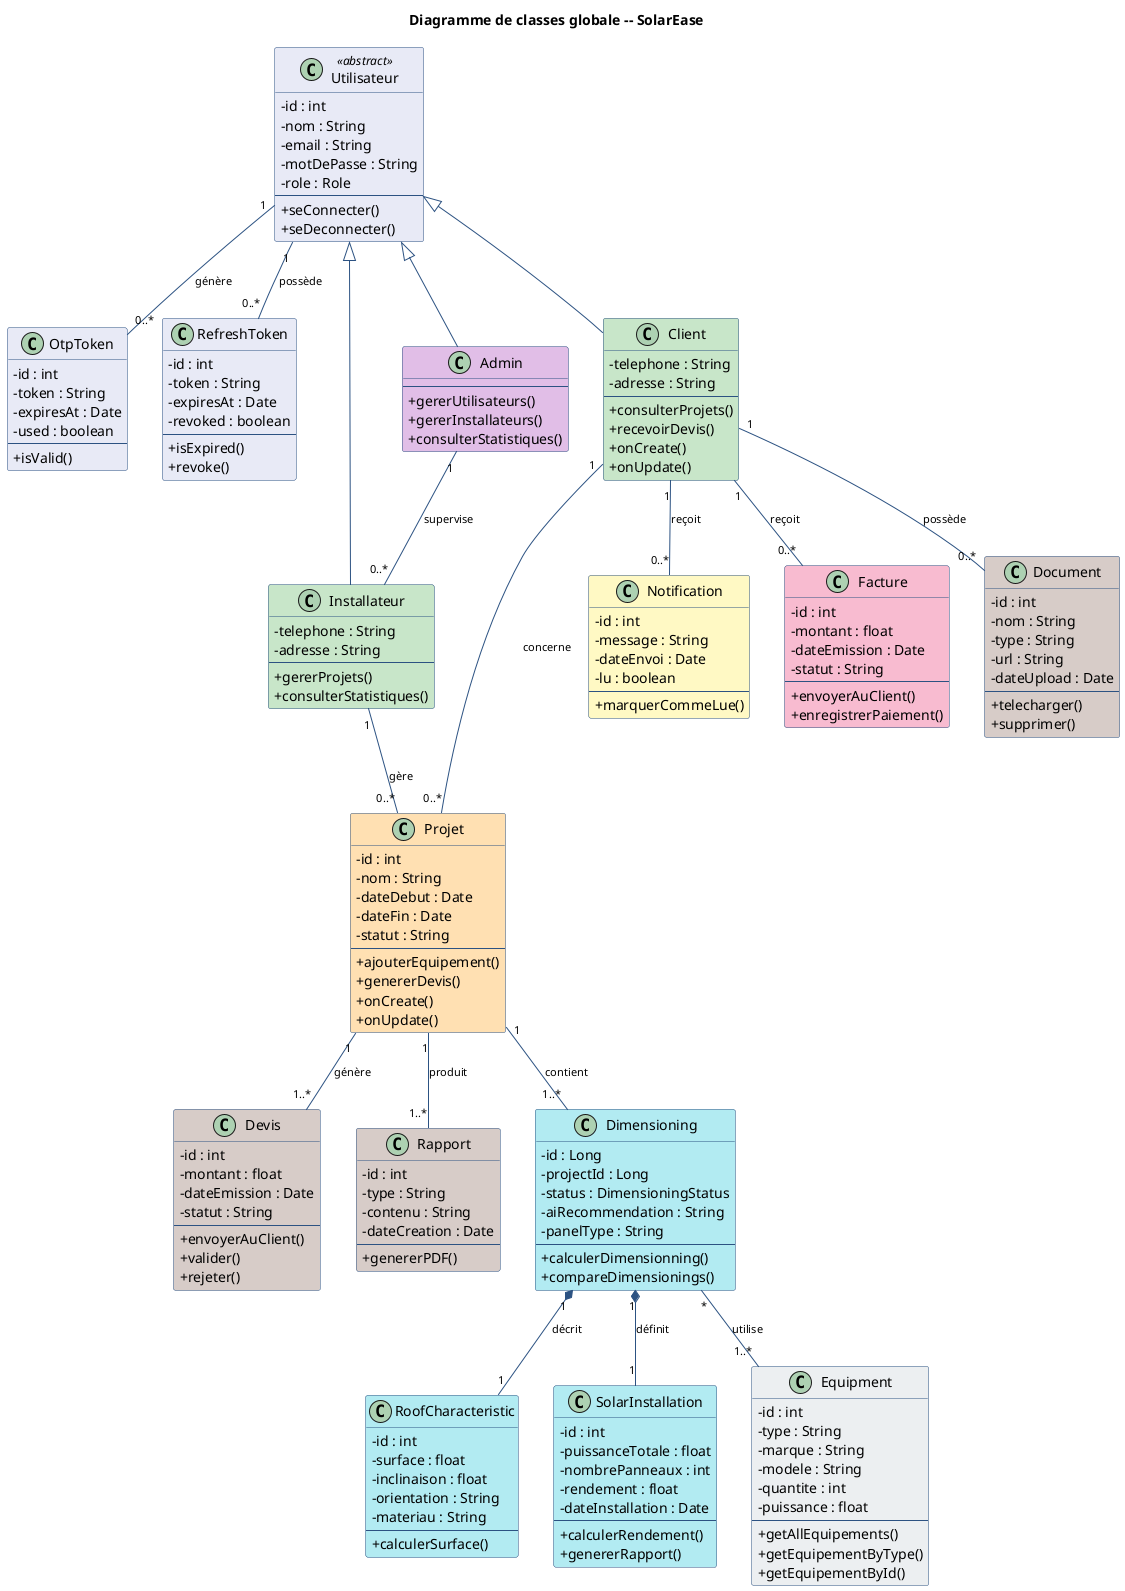
\includegraphics[width=0.92\textwidth]{diagramme-classe-globale.png}
  \caption{Diagramme de classes globale de SolarEase}
  \label{fig:class-diagram}
\end{figure}

\cleardoublepage
